\label{sec:hardsoft}
Our hardware-software co-design DSLAM system contains two essential improvements in the pose estimation and place recognition tasks. As illustrate in \cref{fig:all_us}, both of these two components are divided into two stages: $1)$ CNN front end to extract features which is deployed to the DPU on PL and $2)$ Algebraic operations to present final results which are deployed on the PS ARM cores. To make full use of the Zynq MPSoC, we optimize the data follow for both of these components.

\begin{figure}[t]  
    \centering  
    {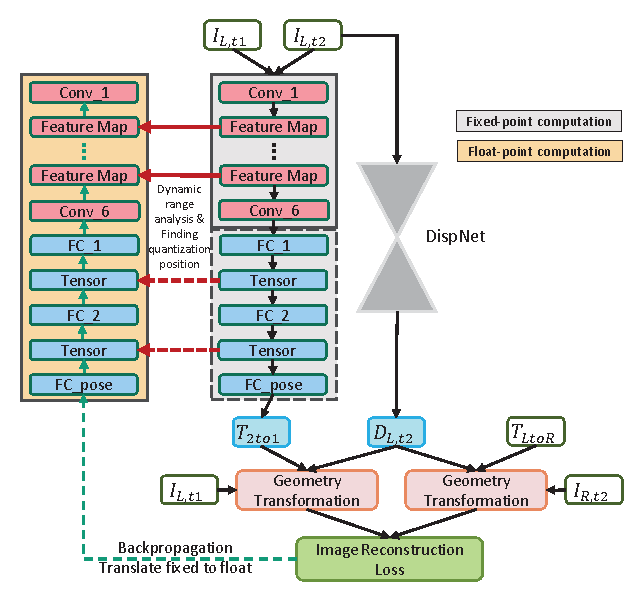
\includegraphics[width=0.8\linewidth]{fig/depth_vo_feat.eps}\label{fig:dvo}}
    \caption{Illustration of training framework for visual odometry, where $T_{LtoR}$ is the relative camera pose transformations between left and right views. To speed up the inference, we attepmt different quantization strategies to fixed-finetune the network for VO with fixed-point feed forwarding and floating-point backpropagation.}
\end{figure}

\subsection{Pose Estimation}
We adopt Depth-VO-Feat \cite{Zhan:2018e92} in DSLAM system to estimate the pose from the input monocular camera. Monocular visual SLAM is a key issue in the field of robotics, while there are two challenging problems: $1)$ it is difficult and expensive to obtain accurate labeled data, $2)$ the methods that use monocular sequences in training always suffer from the scale-ambiguity problem, i.e., the actual scale of translations is missing, and only the direction is learned. In Depth-VO-Feat \cite{Zhan:2018e92}, we use image reconstruction loss as a self-supervised signal to train the convolutional neural networks and jointly train two networks for depth and odometry estimation without external supervision, which can be used independently in the testing phase. Besides, to fix this scale-ambiguity issue, we use stereo sequences in the training phase and monocular sequences in the testing phase. With the known spatial relationship between the left and right cameras, our neural networks can learn the real world scale. Moreover, we use depth smoothness loss to encourage the predicted depth to be smooth, which demonstrated success in prior works. Then the final loss becomes:

\begin{equation}
    L=\lambda_{ir}L_{ir}+\lambda_{ds}L_{ds}
    \label{equ:loss}
\end{equation}

where $L_{ir}$ and $L_{ds}$ are image reconstruction loss and depth smoothness loss respectively, $\lambda_{ir}$ and $\lambda_{ds}$ are the loss weightings for each loss term. The training framework is illustrated in \cref{fig:dvo}.

In order to run our networks efficiently on the FPGA platform, we use fixed-point arithmetic units in the hardware to replace the floating-point number format in GPU and CPU. Many previous works have shown that 8-bit quantization for weights and featuremaps can make the networks run faster on FGPA. Here we adopt the fixed-point finetune method in \cite{Yu:2018:IDC:3299999.3283452}, in that we use the fixed-point number representation in the feed forward phase and keep floating-point number representation for backpropagation, and both weights and data will be re-quantized after each backpropagation. The fixed-point method will lead to a slight accuracy loss of the model, and the performance of the fixed-finetuned Depth-VO-Feat will be shown in detail in \cref{sec:experiment}.

% As the fixed-point method will lead to the accuracy loss of the model, we attempt several different quantization strategies to balance speed and accuracy, which will be shown in detail in \cref{sec:experiment}.

\subsection{Place Recognition}

% \begin{figure}[t]
%     \centering  
%     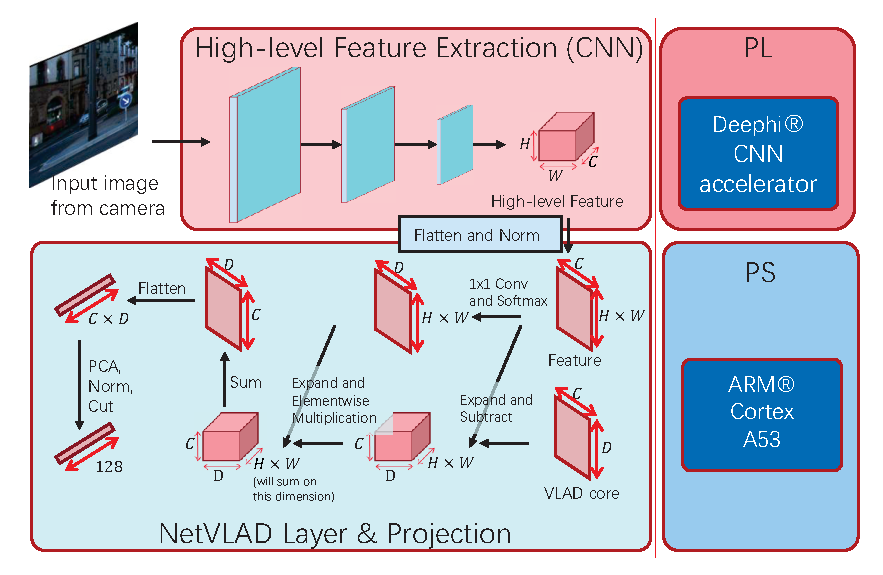
\includegraphics[width=0.95\linewidth]{fig/NetVLAD.eps}
%     \caption{Process of NetVLAD. The CNN encoder is running at the CNN acclerator on PL side, and the VLAD layer as well as the PCA is running at the ARM core at PS side.}
%     \label{fig:NetVLAD}
% \end{figure}

The place recognition method provide the encoded vector transferred to the central agent for inter-robot place matching. As described in \cref{sec:background}, CNN has achieved significant improvements in place recognition tasks, and NetVLAD \cite{Arandjelovic:2017997} is one of the most impressive methods. The CNN-based place recognition methods give the global descriptor of a camera frame in a two-step manner: $1)$ Firstly, a CNN encoder fetches the high-level feature map. $2)$ A vectorization component that aggregates the feature map into a shot global descriptor. The VLAD layer \cite{Arandjelovic:2017997} is a recently proposed plug-and-play operation that greatly improves the performance of place recognition. In the original work with the VLAD layer \cite{Arandjelovic:2017997}, the feature extraction encoder is a typical CNN named VGG-16 \cite{Simonyan:20143be}. The output dimension of original NetVLAD is usually tens of thousands, which is very difficult to be stored on the embedded system, not to mention in the communication-constrained environment. The PCA and the projection method can drastically reduce the output dimension. The previous works\cite{Cieslewski:20187ee} show that 128 dimension is plenty for DSLAM. The data flow and operations of the NetVLAD layer and the projection are complex and require the floating-point number, which cannot be supported with Deephi DPU. We implement the NetVLAD layer and the projection on the PS side of Zynq MPSoC.


Unlike the fixed-point finetune method used for pose estimation. The training procedure with huge non-public datasets is very complicated, and also we cannot finetune the NetVLAD model because of the lack of training data. We simply analyze the dynamic range of the weight and intermediate feature map of each CNN layer and figure out the optimal decimal point position for each layer respectively to minimize the truncation error of each layer.
This method is proposed in \cite{Qiu:2016151} and is used in many tasks such as image classification and image detection.

\subsection{Parallel Scheduling for VO and NetVLAD}

The time consumption of NetVLAD and VO is imbalanced. We do pipeline optimization to schedule the two components on Zynq MPSoC efficiently. The pipeline is illustrated in \cref{fig:pipline}. The interval time for reading camera is $T_{f}$. The CNN time for NetVLAD and VO is $T_{0}$ and $T_{1}$. The computation time cost on PS for VO and NetVLAD is $T_{2}$ and $T_{3}$. We do VO every input frame and do NetVLAD every $N$ frames.

\begin{figure}[t]
    \centering  
    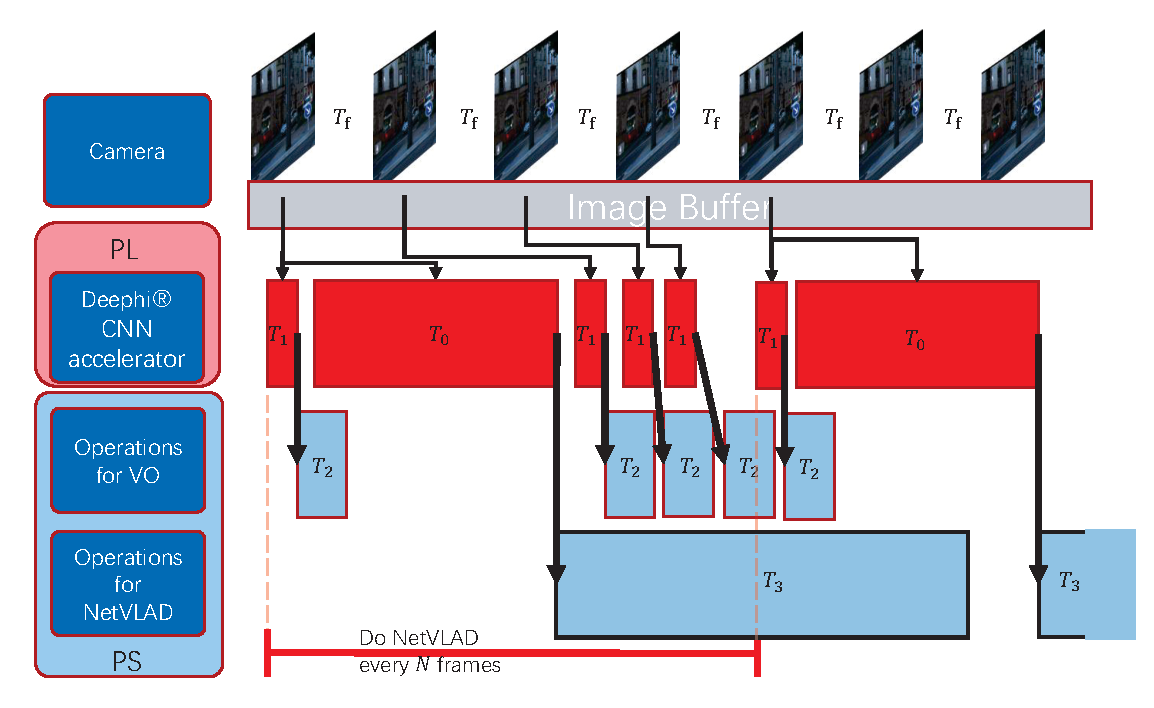
\includegraphics[width=0.95\linewidth]{fig/pipeline.eps}
    \caption{Scheduling pipeline. There are four threads: Camera read, Deephi core at PL, PS Operations for VO, and PS Operations for NetVLAD.}
    \label{fig:pipline}
\end{figure}

% The constrain of these computation time and $N$ is given as \cref{equ:pipline}.

Considering the thread on PL, the time constraint is given as \cref{equ:pipeline1}. 

\begin{equation}
    N \times T_{f} > T_{0} + N \times T_{1}
    \label{equ:pipeline1}
\end{equation}

The thread for VO on PS constrains the NetVLAD frequency as \cref{equ:pipeline2}.

\begin{equation}
    N \times T_{f} > T_{0} + T_{1} + (N-1) \times T_{2}
    \label{equ:pipeline2}
\end{equation}

The PS part of NetVLAD should finish before computing the PS part of next NetVLAD frame. This constraint can be written as \cref{equ:pipeline3}.

% The PS part of NetVLAD should finish before computing the PS part for next NetVLAD frame, and can be writen as \cref{equ:pipline3}.

\begin{equation}
    N \times T_{f} > T_{3}
    \label{equ:pipeline3}
\end{equation}

The execution time of our design will be given in \cref{sec:experiment}.